\documentclass[tikz]{standalone}

\usepackage[T1]{fontenc}
\usepackage{times}

\definecolor{background}{HTML}{ece4d2}

\begin{document}
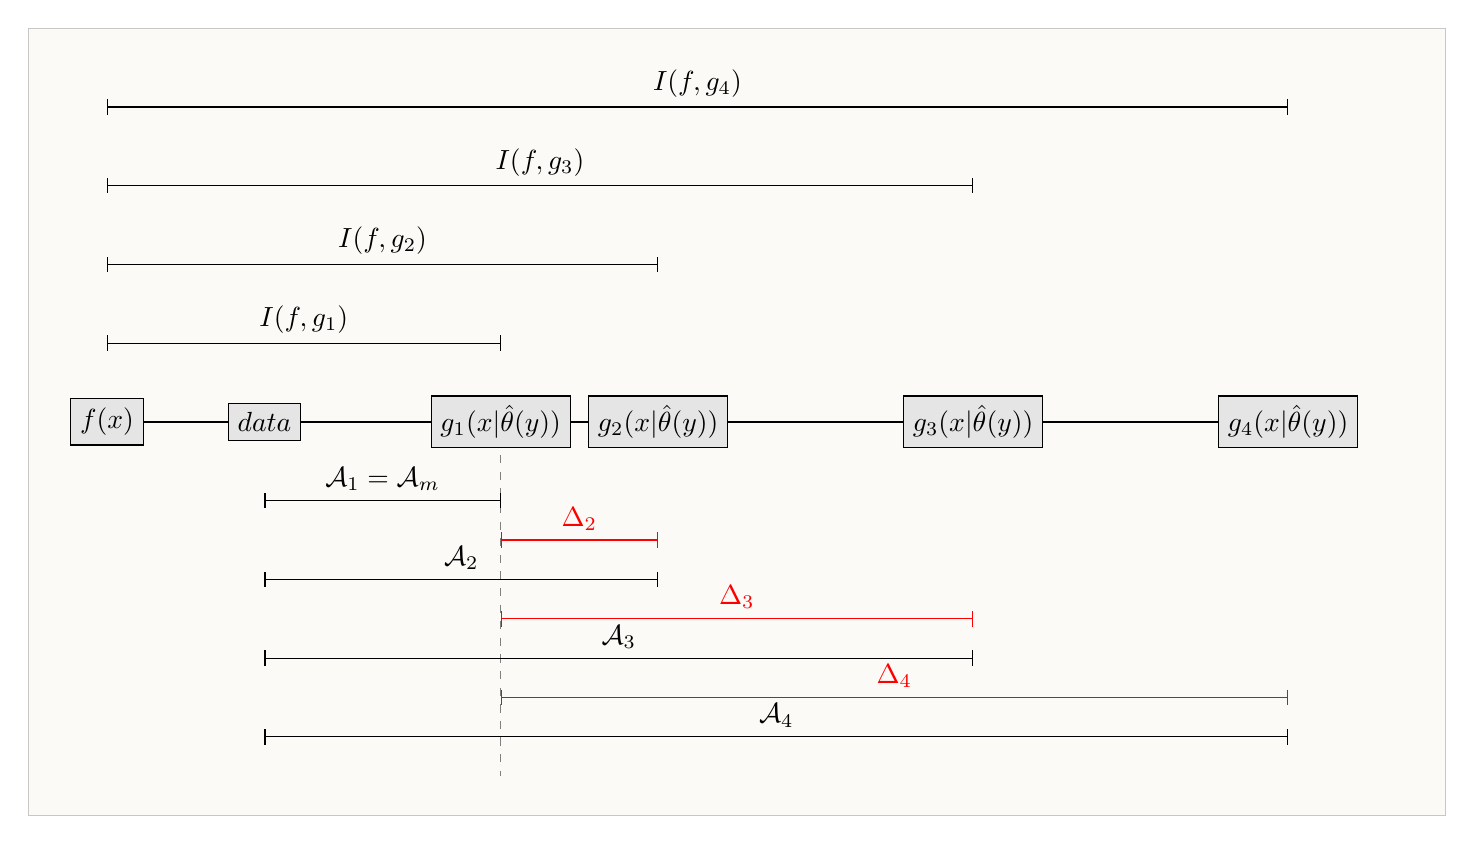
\begin{tikzpicture}

\draw[fill=background, opacity=0.2] (-1,-5) rectangle (17,5);

\draw[line width=1pt] (0,0) -- (15,0);
\draw[dashed, gray] (5,0) -- (5,-4.5);
\node at (0,0) [rectangle, draw, fill=gray!20] {$f(x)$};
\node at (2,0) [rectangle, draw, fill=gray!20] {$data$};
\node at (5,0) [rectangle, draw, fill=gray!20] {$g_1(x|\hat{\theta}(y))$};
\node at (7,0) [rectangle, draw, fill=gray!20] {$g_2(x|\hat{\theta}(y))$};
\node at (11,0) [rectangle, draw, fill=gray!20] {$g_3(x|\hat{\theta}(y))$};
\node at (15,0) [rectangle, draw, fill=gray!20] {$g_4(x|\hat{\theta}(y))$};

\draw[|-|] (0, 1)  -- node [above] {$I(f, g_1)$} (5,1) ;
\draw[|-|] (0, 2)  -- node [above] {$I(f, g_2)$} (7,2) ;
\draw[|-|] (0, 3)  -- node [above] {$I(f, g_3)$} (11,3) ;
\draw[|-|] (0, 4)  -- node [above] {$I(f, g_4)$} (15,4) ;

\draw[|-|] (2, -1)  -- node [above] {$\mathcal{A}_1 = \mathcal{A}_m$} (5,-1) ;
\draw[|-|] (2, -2)  -- node [above] {$\mathcal{A}_2$} (7,-2) ;
\draw[|-|] (2, -3)  -- node [above] {$\mathcal{A}_3$} (11,-3) ;
\draw[|-|] (2, -4)  -- node [above] {$\mathcal{A}_4$} (15,-4) ;

\draw[|-|, red] (5, -1.5)  -- node [above, red] {$\Delta_2$} (7,-1.5) ;
\draw[|-|, red] (5, -2.5)  -- node [above, red] {$\Delta_3$} (11,-2.5) ;
\draw[|-|, red] (5, -3.5)  -- node [above, red] {$\Delta_4$} (15,-3.5) ;



\end{tikzpicture}
\end{document}
